\documentclass{article}
\usepackage[utf8]{inputenc}
\usepackage{tasks}
\usepackage{amsthm}
\usepackage{amssymb}
\usepackage{hyperref}
\usepackage{mathtools}
\usepackage{cleveref}
\usepackage{lipsum}
\usepackage{polynom}
\usepackage{array}
\usepackage{algorithm}
\usepackage{algpseudocode}
\usepackage{physics}
\usepackage{tikz}
\newtheorem{theorem}{Theorem}
\newtheorem{lemma}{Lemma}
\newtheorem{define}{Definition}
\newtheorem{problem}{Problem}
\title{Computational Geometry in Minecraft: Integer Block Ray Shooting Problem}
\author{ANEP Research}
\begin{document}
\maketitle
\tableofcontents
\section{Introduction}
\begin{define}
    \textbf{Block} in block space $\mathbb{R}^{3}$ is a integer polytope cube and length of each edges is $1$.
\end{define}
\begin{define}
    \textbf{Block space} $\mathcal{B}(w,h,r)$ is a $w \times h \times r$ integer polytope cube in euclidean space $\mathbb{R}^{3}$.
\end{define}
\begin{problem}
    \label{ibrs}
    \textbf{Integer block ray shooting problem} in block space $\mathcal{B}(w,h,r)$ is
    decide if there exists a block $B \in \mathcal{B}(w,h,r)$ which intersects in $intB$ by a vector $\vec{l} = (x, \frac{h}{w}x, \frac{r}{w}x))$.
\end{problem}
We shall introduce an efficient algorithm to solve \cref{ibrs}.
\pagebreak
\section{Efficient algorithm: IBRS Problem}
\begin{algorithm}
    \caption{IBRS Problem in $O(n)$ time}\label{ibrs_algorithm}
    \begin{algorithmic}[1]
        \Procedure{IBRS}{$\mathcal{B}(w,h,r)$}\Comment{A block space $\mathcal{B}(w,h,r)$}
            \For{$i \gets 1$ to $w$}
                \State $\vec{l}_{i} \gets (i,\lfloor \frac{h}{w} i \rfloor,\lfloor \frac{r}{w} i \rfloor)$
                \If{CheckBlock($\vec{l}_{i}$)}\Comment{Procedure CheckBlock($\vec{v}$) is checking if there is an block at position $\vec{v}=(x,y,z)$ to $(x+1,y+1,z+1)$ in the block space $\mathcal{B}$}
                    \State \textbf{return} $false$
                \EndIf
            \EndFor
            \For{$j \gets 1$ to $h$}
                \State $\vec{l}_{j} \gets (\lfloor \frac{w}{h} j \rfloor,j,\lfloor \frac{r}{h} j \rfloor)$
                \If{CheckBlock($\vec{l}_{j}$)}
                    \State \textbf{return} $false$
                \EndIf
            \EndFor
            \State \textbf{return} true
        \EndProcedure
    \end{algorithmic}
\end{algorithm}
For example, we consider the 2D block space. \\
\begin{center}
    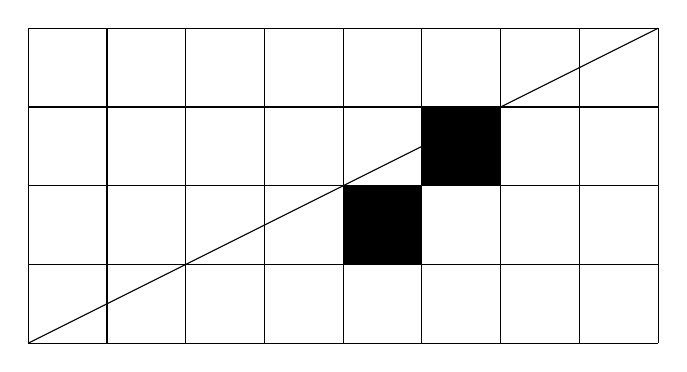
\begin{tikzpicture}
        \draw[step=1cm,black] (0,0) grid (8,4);
        \draw[black] (0,0) -- (8,4);
        \fill[black] (4,1) rectangle (5,2);
        \fill[black] (5,2) rectangle (6,3);
    \end{tikzpicture}
\end{center}
And we may process \cref{ibrs_algorithm} in this 2D block space.
For the first loop in line 2, there is nothing happended until $i=5$.
We consider $i=5$, $\vec{l}_{i} = (5, 0, 2)$ and the result of $CheckBlock(\vec{l}_{i})$ is $true$.
Thus, the result of algorithm is $false$. \\ \\
And we are going to proof the correctness of \cref{ibrs_algorithm}.
\begin{lemma}
    \label{lem1}
    $(i,\frac{h}{w} i,\frac{r}{w} i)$ and $(\frac{w}{h} j,j,\frac{r}{h} j)$ are same straight line in $\mathbb{R}^{3}$.
\end{lemma}
\begin{proof}
    If $i=0$ then $(i,\frac{h}{w} i,\frac{r}{w} i)=(0,0,0)$ 
    and $i=w$ then $(w, h, r)$.
    And if $j=0$ then $(\frac{w}{h} j,j,\frac{r}{h} j)=(0,0,0)$
    and $j=h$ then $(w,h,r)$.
    Thus both straight line pass two points.
    Since first axiom of euclidean geomtry, Both straight lines are same.
\end{proof}
\begin{theorem}[Correctness of \cref{ibrs_algorithm}]
    An \cref{ibrs_algorithm} correctly decides \cref{ibrs}.
\end{theorem}
\begin{proof}
    Firstly, We consider lines 2-7 of \cref{ibrs_algorithm}.
    \begin{center}
        \begin{tikzpicture}
            \draw[black] (0,0) rectangle (2,2);
            \draw[blue] (-1,0) -- (3,2);
        \end{tikzpicture}
    \end{center}
    If a line and a square meet as shown in the photo, the point where it first meets is $(x_{0},y_{0},z_{0})$, 
    then it's trivial the point left-bottom vertex of square is $(x_{0},\lfloor y_{0} \rfloor,\lfloor z_{0} \rfloor)$.
    And it is $(x, \lfloor \frac{h}{w} x \rfloor, \lfloor \frac{r}{w} x \rfloor)$. 
    When $i=x$ in the loop lines 2-7, Since line 4, It checks whether there is block which is intersected by a line.
    That is, If $\vec{l}_{i}$ implies left-bottom vertex of square, A line intersects with a square.
    If it is not true, which is contradicting to first axiom of euclidean geometry.
    And lines 8-13 is the case when $y$-coordinate is always integer. \\
    Since \cref{lem1}, It considers same straight line in lines 2-7 and lines 8-13.
    It can also be proved in the same way. \\
    Then it is all possible cases about the position of block in a block space $\mathcal{B}$. \\
    Thus \cref{ibrs_algorithm} correctly decides \cref{ibrs}.
\end{proof}
\begin{theorem}[Complexity of \cref{ibrs_algorithm}]
    An \cref{ibrs_algorithm} has $O(\max(w,h))$ time complexity and $O(1)$ space complexity.
\end{theorem}
\begin{proof}
    Straightfoward.
\end{proof}
\end{document}